\documentclass[12pt]{article}

\usepackage{amsmath, float, graphicx, hyperref}

\begin{document}
\title{Numerically Solving Continuity Equations}
\author{Carl Denton}
\maketitle

\section{Introduction}

Continuity equations are of interest for a variety of reasons, the most important of which is that they model a wide range of physical phenomena including conservation of mass in fluids. However, they are generally far more difficult to solve than the closely related Advection-Diffusion equations due to the fact that they have no diffusive term and are thus far more unstable. 

Here we implement the upwind and SHASTA methods for solving these equations and test a number of their initial conditions. 

\vspace{1pc}

\noindent Code at \url{https://github.com/cfdenton/ac274} in continuity.py

\section{Problem}

The continuity equation is given by
\[\frac{\partial}{\partial t} \varphi + \nabla\cdot \vec J[\varphi] = S\]
for flux $\hat J$, density $\varphi$, and source $S$. We focus here on flux of the form
\[\vec J[\varphi] = \vec u(x, t)\varphi - D(x)\nabla \varphi\]
This equation becomes particularly difficult to solve for $D = 0$, as the lack of diffusion makes it much harder to maintain stability.


\section{Methods}

\subsection{Upwind Finite Differences}
The first method we explore is the upwind finite differences scheme. This is similar to standard centered finite-differences, with the main difference being that the spatial derivatives are one-sided, in the direction of positive advection. 
That is, to solve the continuity equation
\[\frac{\partial}{\partial t}\varphi = -\frac{\partial}{\partial x} u(x)\varphi\]
we use the scheme
\[\frac{\varphi_j^{n+1}-\varphi_j^n}{h} = \begin{cases} \frac{u_{j}\varphi_j^n - u_{j-1}\varphi_{j-1}^n}{d} & \text{ if } u_j \geq 0 \\ \frac{u_{j+1}\varphi^n_{j+1} - u_j\varphi^n_j}{d} & \text{ if } u_j < 0\end{cases} \]
This is typically quite stable--- unfortunately, this stability comes at the cost of high degrees of numerical diffusion.

\subsection{SHASTA}

The second method we implement is the SHASTA algorithm, a type of flux-corrected transport. 
The essential intuition of the algorithm is to move each grid point with the motion of the fluid, and then interpolate the results back to the original grid. Finally an antidiffusive term is added to compensate for the excess numerical diffusion created in the process.
The result is an algorithm of the form 
\[\varphi_j^{n+1} = \frac{1}{2}Q_{-}^2 \left(\varphi^n_{j-1} - \varphi^n_{j}\right) + \frac{1}{2}Q_{+}^2 \left(\varphi_{j+1}^n - \varphi_{j}^n\right) + (Q_{+} + Q_{-})\varphi_j^n\]
where
\[Q_{\pm} = \left(\frac{1}{2} \mp u_j \frac{h}{d}\right)\big/\left[1 \pm (u_{j \pm 1} - u_j)\frac{h}{d}\right]\]
followed by an antidiffusive term given by
\[\bar \varphi_j^n = \varphi_j^n - f_{j + 1/2} + f_{j - 1/2}\]
where 
\[f_{j + 1/2} = \text{sgn } \Delta_{j+ 1/2} \max \left\{0, \min\left\{\Delta_{j-1/2}\text{ sgn }\Delta_{j+1/2}, \frac{1}{8}\left|\Delta_{j+1/2} \right|, \Delta_{j+3/2}\text{ sgn }\Delta_{j+1/2}\right\}\right\}\]
and $f_{j-1/2}$ is obtained by setting $j \rightarrow j-1$. This set of conditions ensures positivity while eliminating excess diffusion. The authors of the original paper note that further accuracy can be achieved by modifying the $\frac{1}{8}$ term.

\section{Experiments}

\subsection{Upwind}

We first test the method with gaussian and box initial conditions, under spatially uniform advection.
The results are plotted below.
\begin{figure}[H]
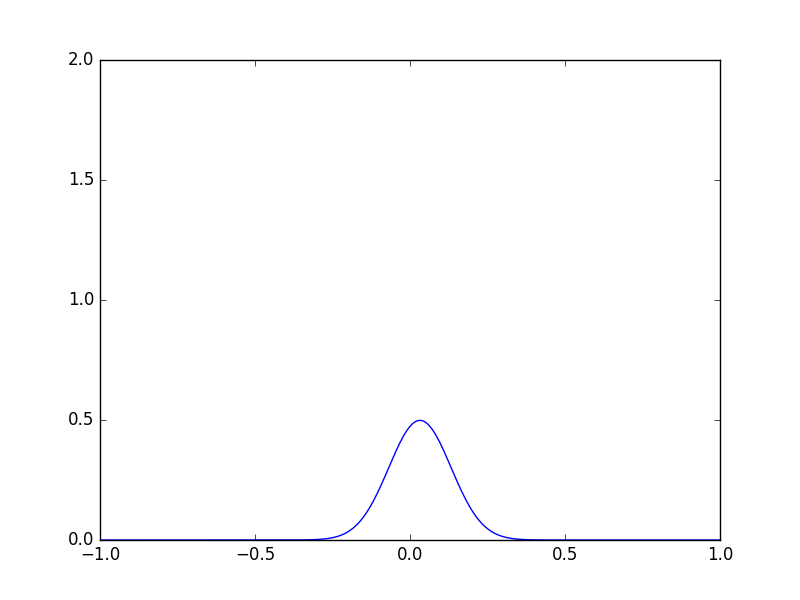
\includegraphics[width = .32\hsize]{gaussian_upwind_init.png} 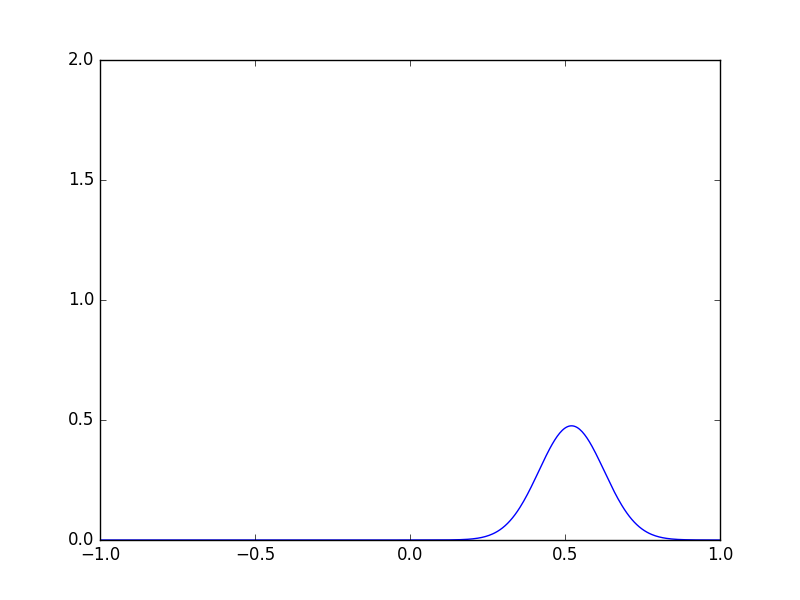
\includegraphics[width = .32\hsize]{gaussian_upwind_2.png} 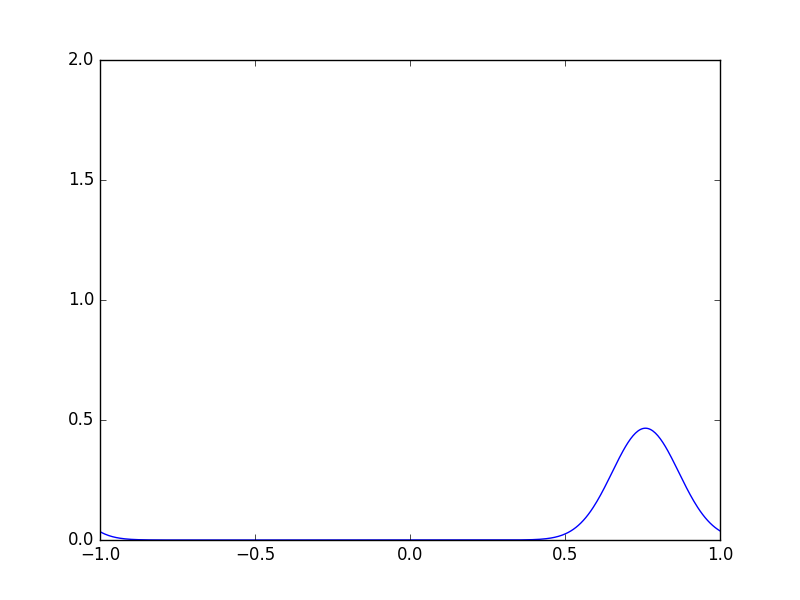
\includegraphics[width = .32\hsize]{gaussian_upwind_3.png}
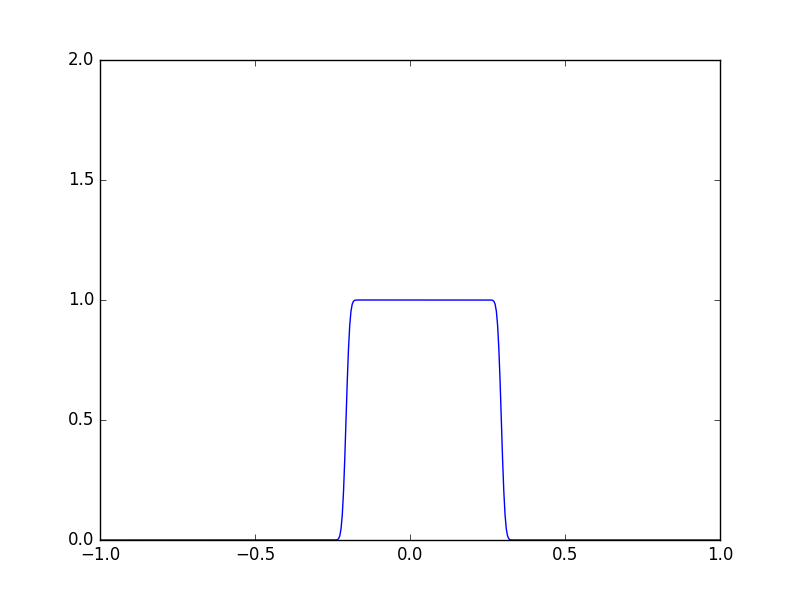
\includegraphics[width = .32\hsize]{box_upwind_1.png} 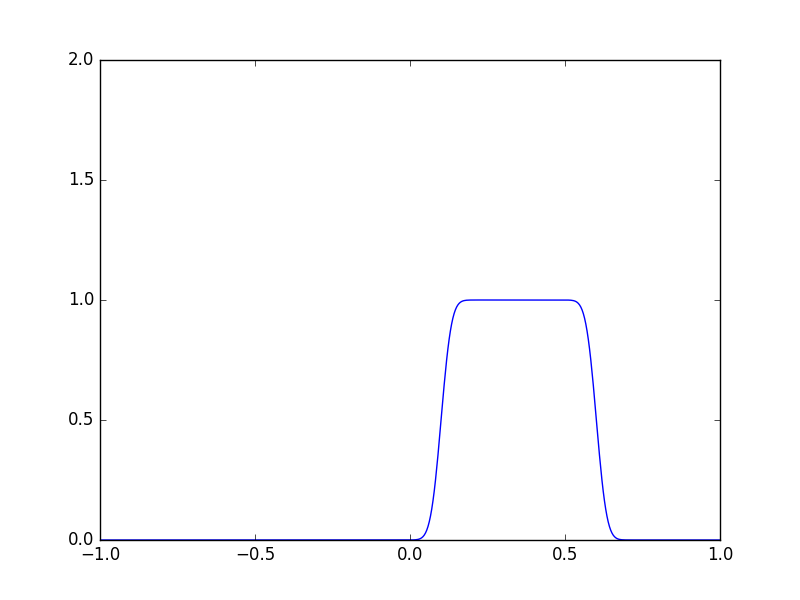
\includegraphics[width = .32\hsize]{box_upwind_2.png} 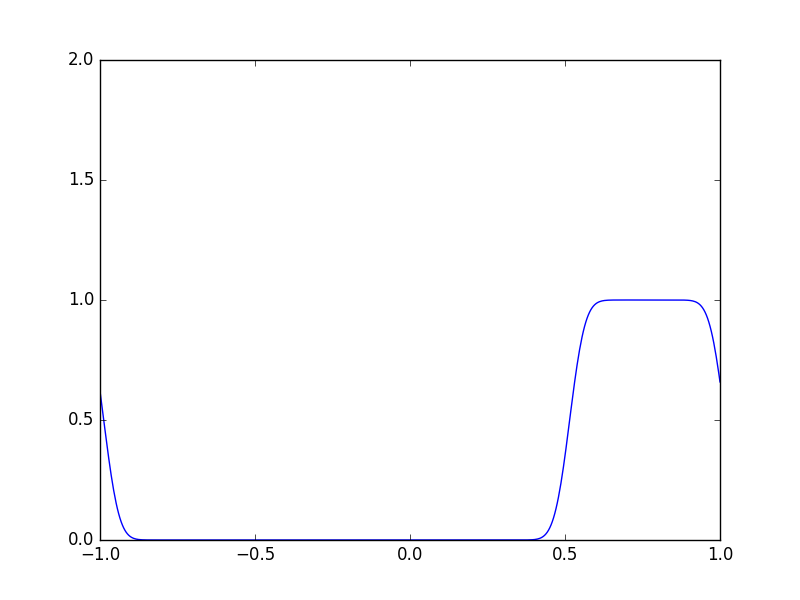
\includegraphics[width = .32\hsize]{box_upwind_3.png}
\end{figure}
Note the numerical diffusion, particularly noticeable in the case of a box wave, which appears as a side effect of the method. 

\subsubsection{Validation}

We perform a grid convergence analysis by running the simulation with uniform advection for grid sizes $N$ and $2N$, where $N = 10, \dots, 2000$. The root-mean-square error of the result at time step $t = 100$ between the simulation on a grid of size $N$ and a grid of size $2N$ is plotted below.
Clearly the solution converges quite well for fine meshes.
\begin{figure}[H]
\begin{center}
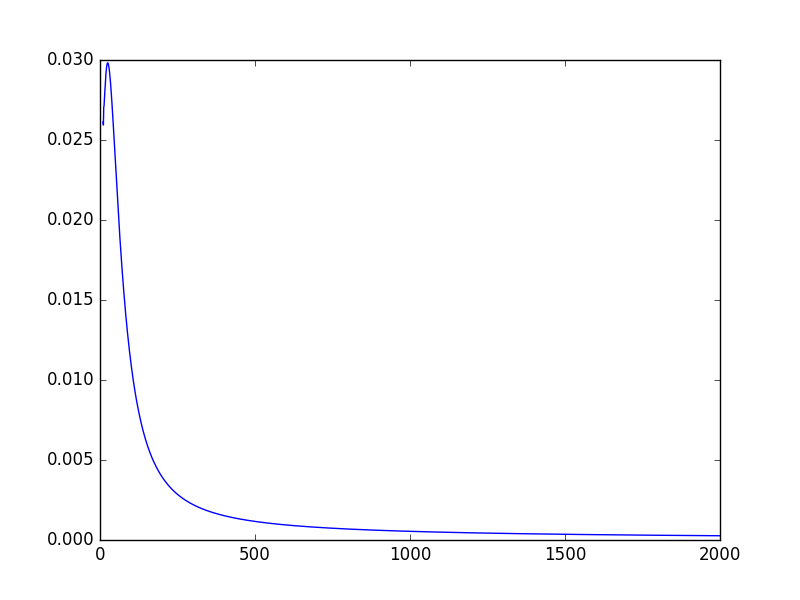
\includegraphics[width = .85\hsize]{upwind_convergence.png}
\end{center}
\end{figure}

\subsection{SHASTA}

We perform the same experiments using the SHASTA method, with the results shown below.
In this case numerical diffusion plays a far lesser role; the box wave can be seen to maintain its shape almost perfectly.
\begin{figure}[H]
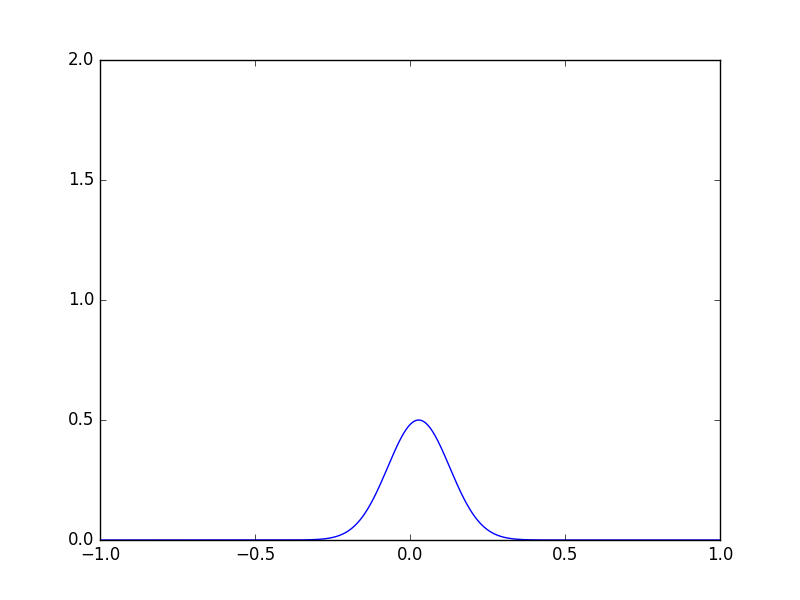
\includegraphics[width = .32\hsize]{shasta_gaussian_1.png} 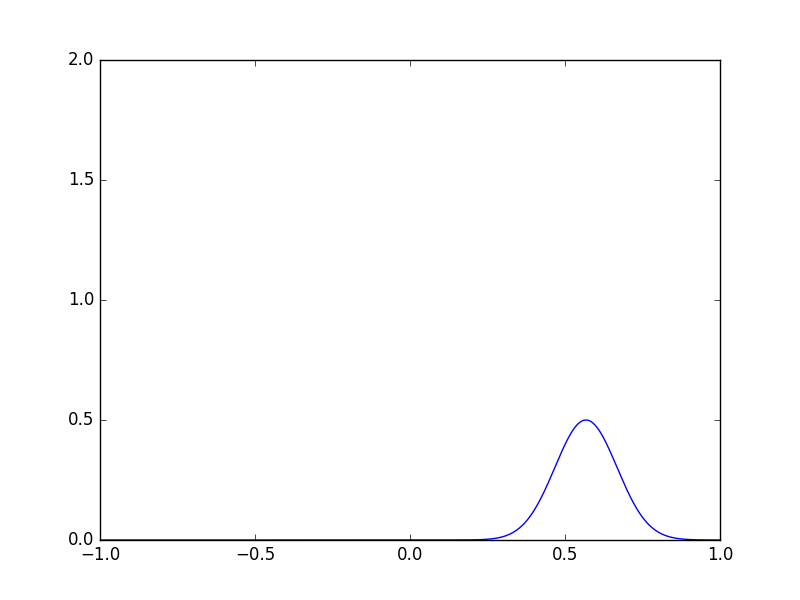
\includegraphics[width = .32\hsize]{shasta_gaussian_2.png} 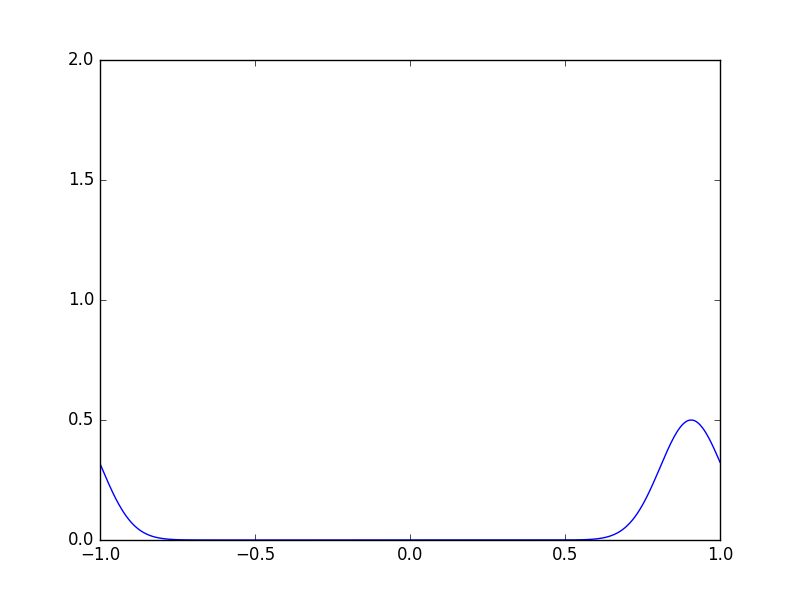
\includegraphics[width = .32\hsize]{shasta_gaussian_3.png}
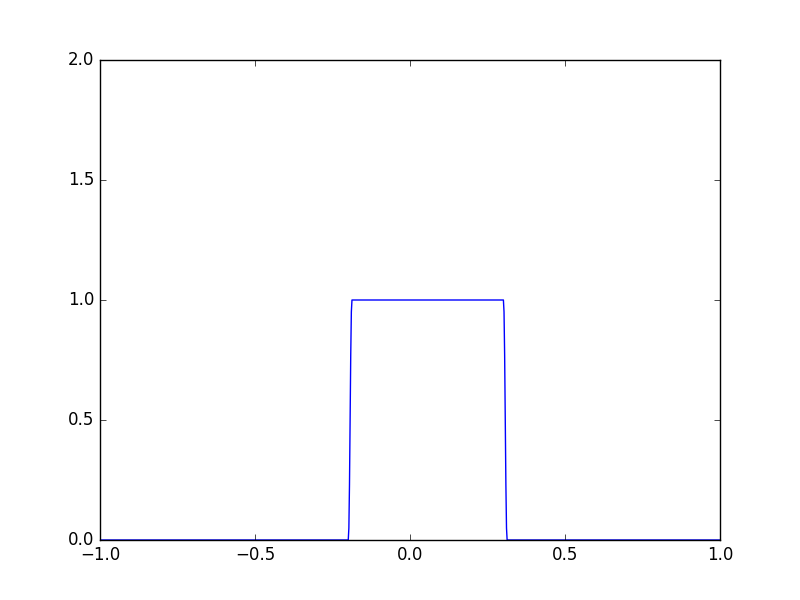
\includegraphics[width = .32\hsize]{shasta_box_1.png} 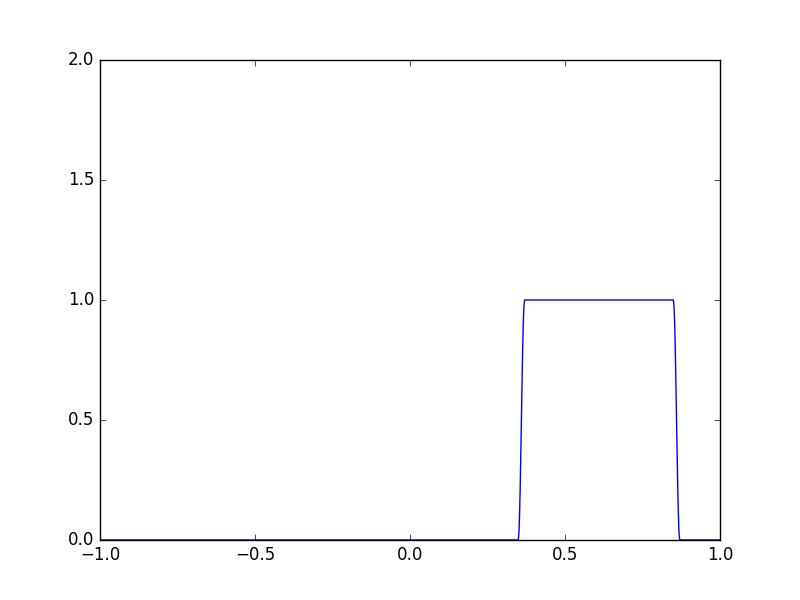
\includegraphics[width = .32\hsize]{shasta_box_2.png} 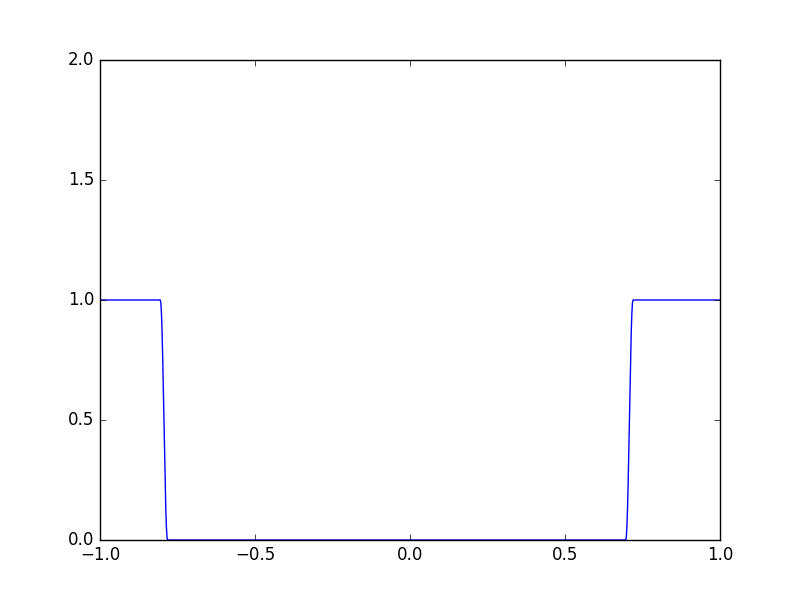
\includegraphics[width = .32\hsize]{shasta_box_3.png}
\end{figure}

\subsubsection{Validation}

We perform a grid convergence analysis identical to the one for the upwind method, with the following results:
\begin{figure}[H]
\begin{center}
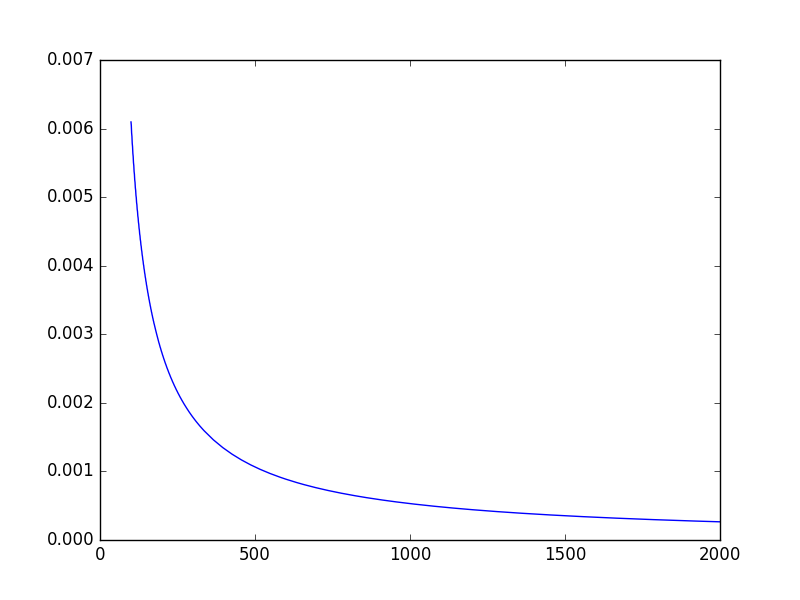
\includegraphics[width = .85\hsize]{shasta_convergence.png}
\end{center}
\end{figure}
\noindent Again, the solutions converge well.
\end{document}
